  \section{Optimisation}

  \subsection{Problem Formulation}
  \begin{frame}
  \frametitle{Problem Formulation}
  \begin{block}{Constrained optimisation problem}
  \begin{equation}
	\begin{cases}
  \mathop{Min}\limits _{(r,R)\in \mathcal{D}} \alpha C(r,R) + \beta Vol(r,R) \\
  C(r,R) \leq C_s\\
  2 \leq Q(r,R) \leq 4
	\end{cases}
  \end{equation}
  \end{block}

  \begin{itemize}
  \item $ \mathcal{D} = [2,6] \times [7,20]$
  \item  \emph{Vol} represents the volume of the device
  \item  $\alpha$ and $\beta$ weights on concentration and volume
  \item The dimension of the radius is the millimetre.\\
  \item We use $\Delta p = kQ^2$ to have the constraint on the flow.
  \end{itemize}
  \end{frame}

  \subsection{First Approximation}
  \begin{frame}
  \frametitle{First Approximation : $\beta = 0$}
  \begin{block}{Our optimisation problem}
$$ 
\begin{cases}
\mathop{\rm Min}\limits _{(r,R)} c(r,R) & = c_0 \exp{(-kI\frac{z}{U(r,R)})}\\
Q_1(r,R) & = 2-\pi r_{exit}^2U(r,R) \leq 0 \\
Q_2(r,R) & = \pi r_{exit}^2U(r,R) - 4 \leq 0
\end{cases}
$$
  \end{block}
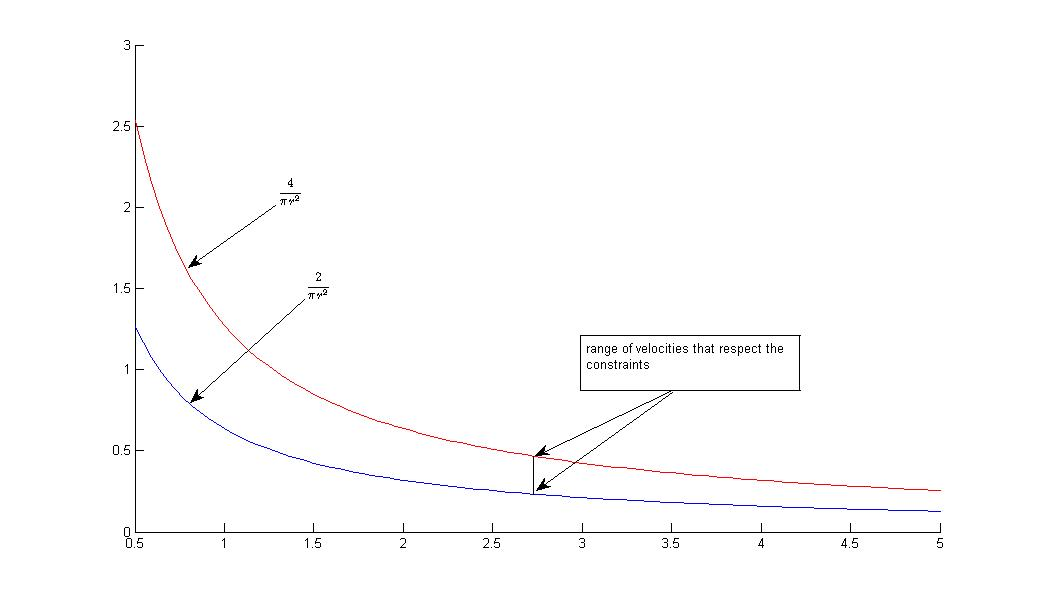
\includegraphics[height=4cm, width=5cm]{images/vrange.jpg}
\hspace{0.2cm}
\begin{minipage}{5cm}
$\frac{2}{\pi r^2} \leq U(r,R) \leq \frac{4}{\pi r^2}$
\end{minipage}
  \end{frame}

  \subsection{Second Approximation}
  \begin{frame}
  \frametitle{Second Approximation : $\beta = 0$ and $r=2mm$ $\Rightarrow \mathop{Min}\limits _{R\in [7,20]} C(R)$}
  \begin{block}{Formula}
  \begin{equation}
  \left(f_1(v)\frac{L_1+L_3}{2r} + f_2(v,R)\frac{L_2}{2R} + K_e + K_c\right)\cdot \frac{\rho v^2}{2} - \Delta p = 0
  \end{equation}
  \begin{equation}
  c(R) = c_0\cdot e^{-kI\frac{L_2}{v(R)}}
  \end{equation}
  \end{block}
  $1^{st}$ Step : $v(R)$ \hspace{40mm} $2^{nd}$ Step : $C(R)$
          \begin{figure}
          \raggedleft
          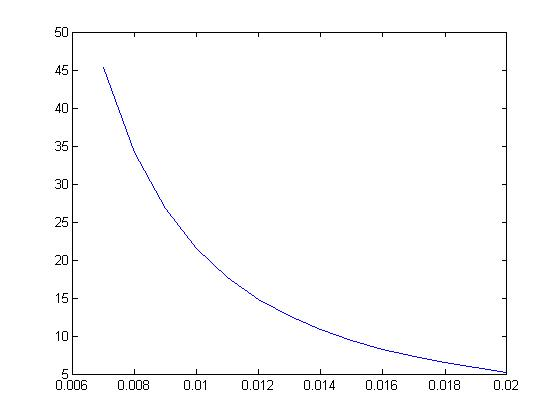
\includegraphics[height=3.1cm, width=5cm]{./images/graphVR.jpg}
          \hspace{5mm}
          \raggedright
          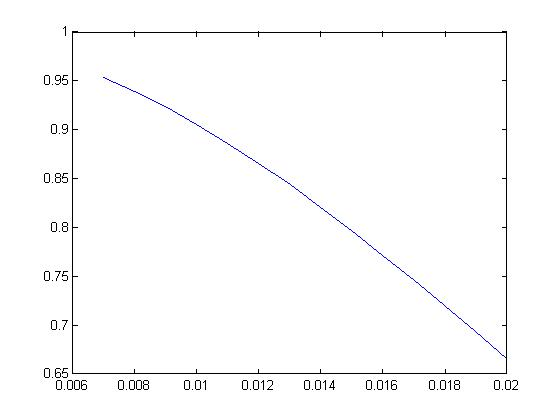
\includegraphics[height=3.1cm, width=5cm]{./images/graphCR.jpg}
          \end{figure}
  \end{frame}

  \subsection{In the Future}
  \begin{frame}
  \frametitle{In the Future}
  \begin{itemize}
  \item 0 Space Dimension :
          \begin{itemize} 
                  \item[*] To find the minimum bacteria concentration with $r$ and $R$.
                  \item[*] To optimize with the volume
          \end{itemize}
  \vspace{1cm}
  \item 1 Space Dimension
  \vspace{1cm}
  \item 2 Space Dimension

  \end{itemize}
  \end{frame}
